%% Lee
%% In dissertation, change 
%    section* to chapter 
%    subsection* to section
%    subsubsection* to subsection

% >>>>>>>>>>>>>>>>>>>>>>>>>>>>>>>>>>>>>>>>>>>>>>>>>>>>>>>>>>>>>>>>>>>>>>>>>>>>> DRAM Customizable <<<<<<<<<>>>>>>>>>>>>>>>>>>>>>>>>>>>>>>>>>>>>>>>>>>>>>>>>>><<<<<<<<<<<<<
\chapter{DRAM Customizations}
\label{sec:DRAM Customizations}

Accessing a typical \acl{sram}, or \ac{sram} involves providing an address and either reading or writing the contents of that location. The read or write often completes in one or two clock cycles depending on whether the \ac{sram} employs internal registers which are used run the \ac{sram} with a faster clock.
The memory cell inside the \ac{sram} is formed from cross-coupled transisters, often six which latch the contents and hold the contents indefnitely or until power is removed from the device.
The structure of the storage element allows the access logic to be relatively simple and fast but has a relatively low capacity.

Accessing a "typical" DRAM is much more involved, it involves opening a page in a bank, reading or writing a portion of the contents of the page then closing the page. 

Typically a bank may contain of the order of a few thousand pages and a page may contain of the order of a few thousand bits.

Once the page is open, the user accesses a portion of the requested page over a bus. With PCB based DRAMs the bus might vary from four to 16 bits wide, but with 3D DRAMs, such as HBM the bus might be up to 128 bits wide.

Figure \ref{fig:dramBlockDiagram} shows a block diagram of a typical DRAM.

\begin{figure}[!t]
% the [] contains position info e.g. [!t] means here
\centering
\captionsetup{justification=centering}
\centerline{
\mbox{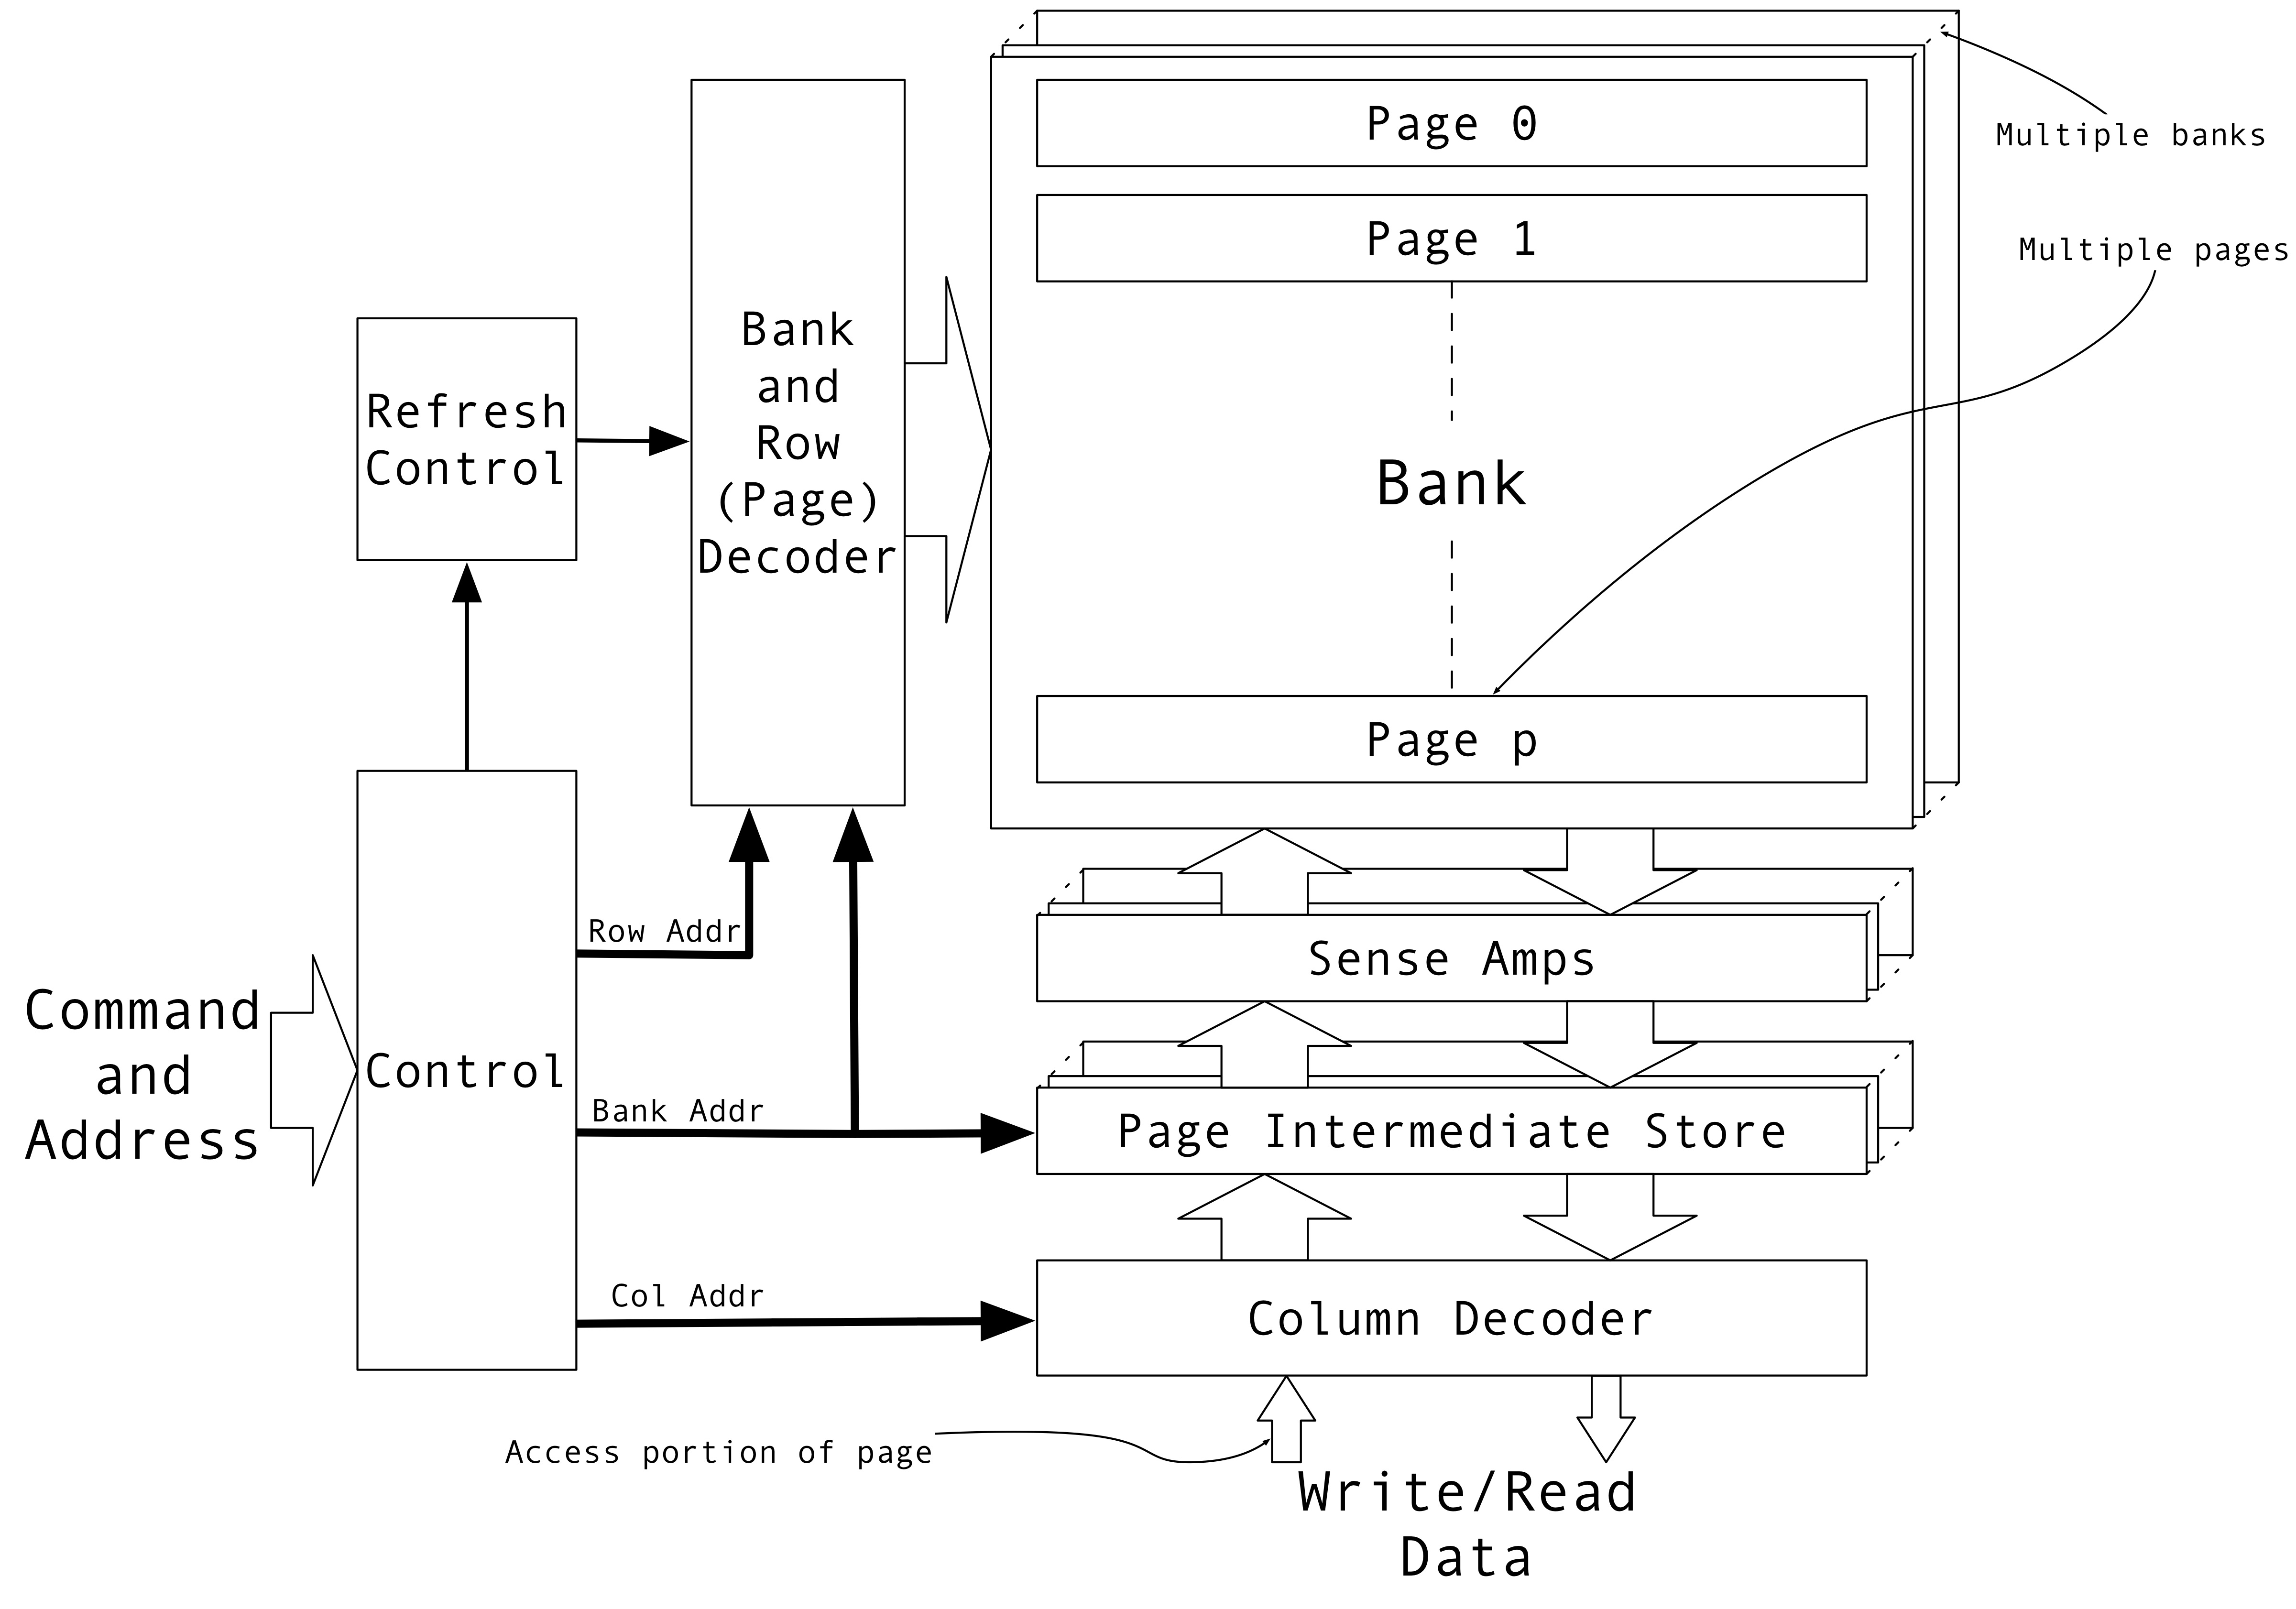
\includegraphics[width=.9\linewidth]{DRAMBlockDiagram.jpg}}
}
\caption{Typical DRAM Block Diagram}
\label{fig:dramBlockDiagram}
\end{figure}

\section{Very-Wide Bus}
\label{sec:Very-Wide Bus}

This work achieves the increase in bandwidth by proposing that the DRAM expose more of its currently open page.

Without the limitations of having to transfer data beyond the chip stack, this work suggests exposing a larger portion of the page over a very wide bus. By staying within the 3D footprint, this bus can be implemented using fine pitch through-silicon-vias.
(see figure \ref{fig:dramBusChange}).

\begin{figure}[!t]
% the [] contains position info e.g. [!t] means here
\centering
\captionsetup{justification=centering}
\captionsetup{width=.9\linewidth}
\centerline{
\mbox{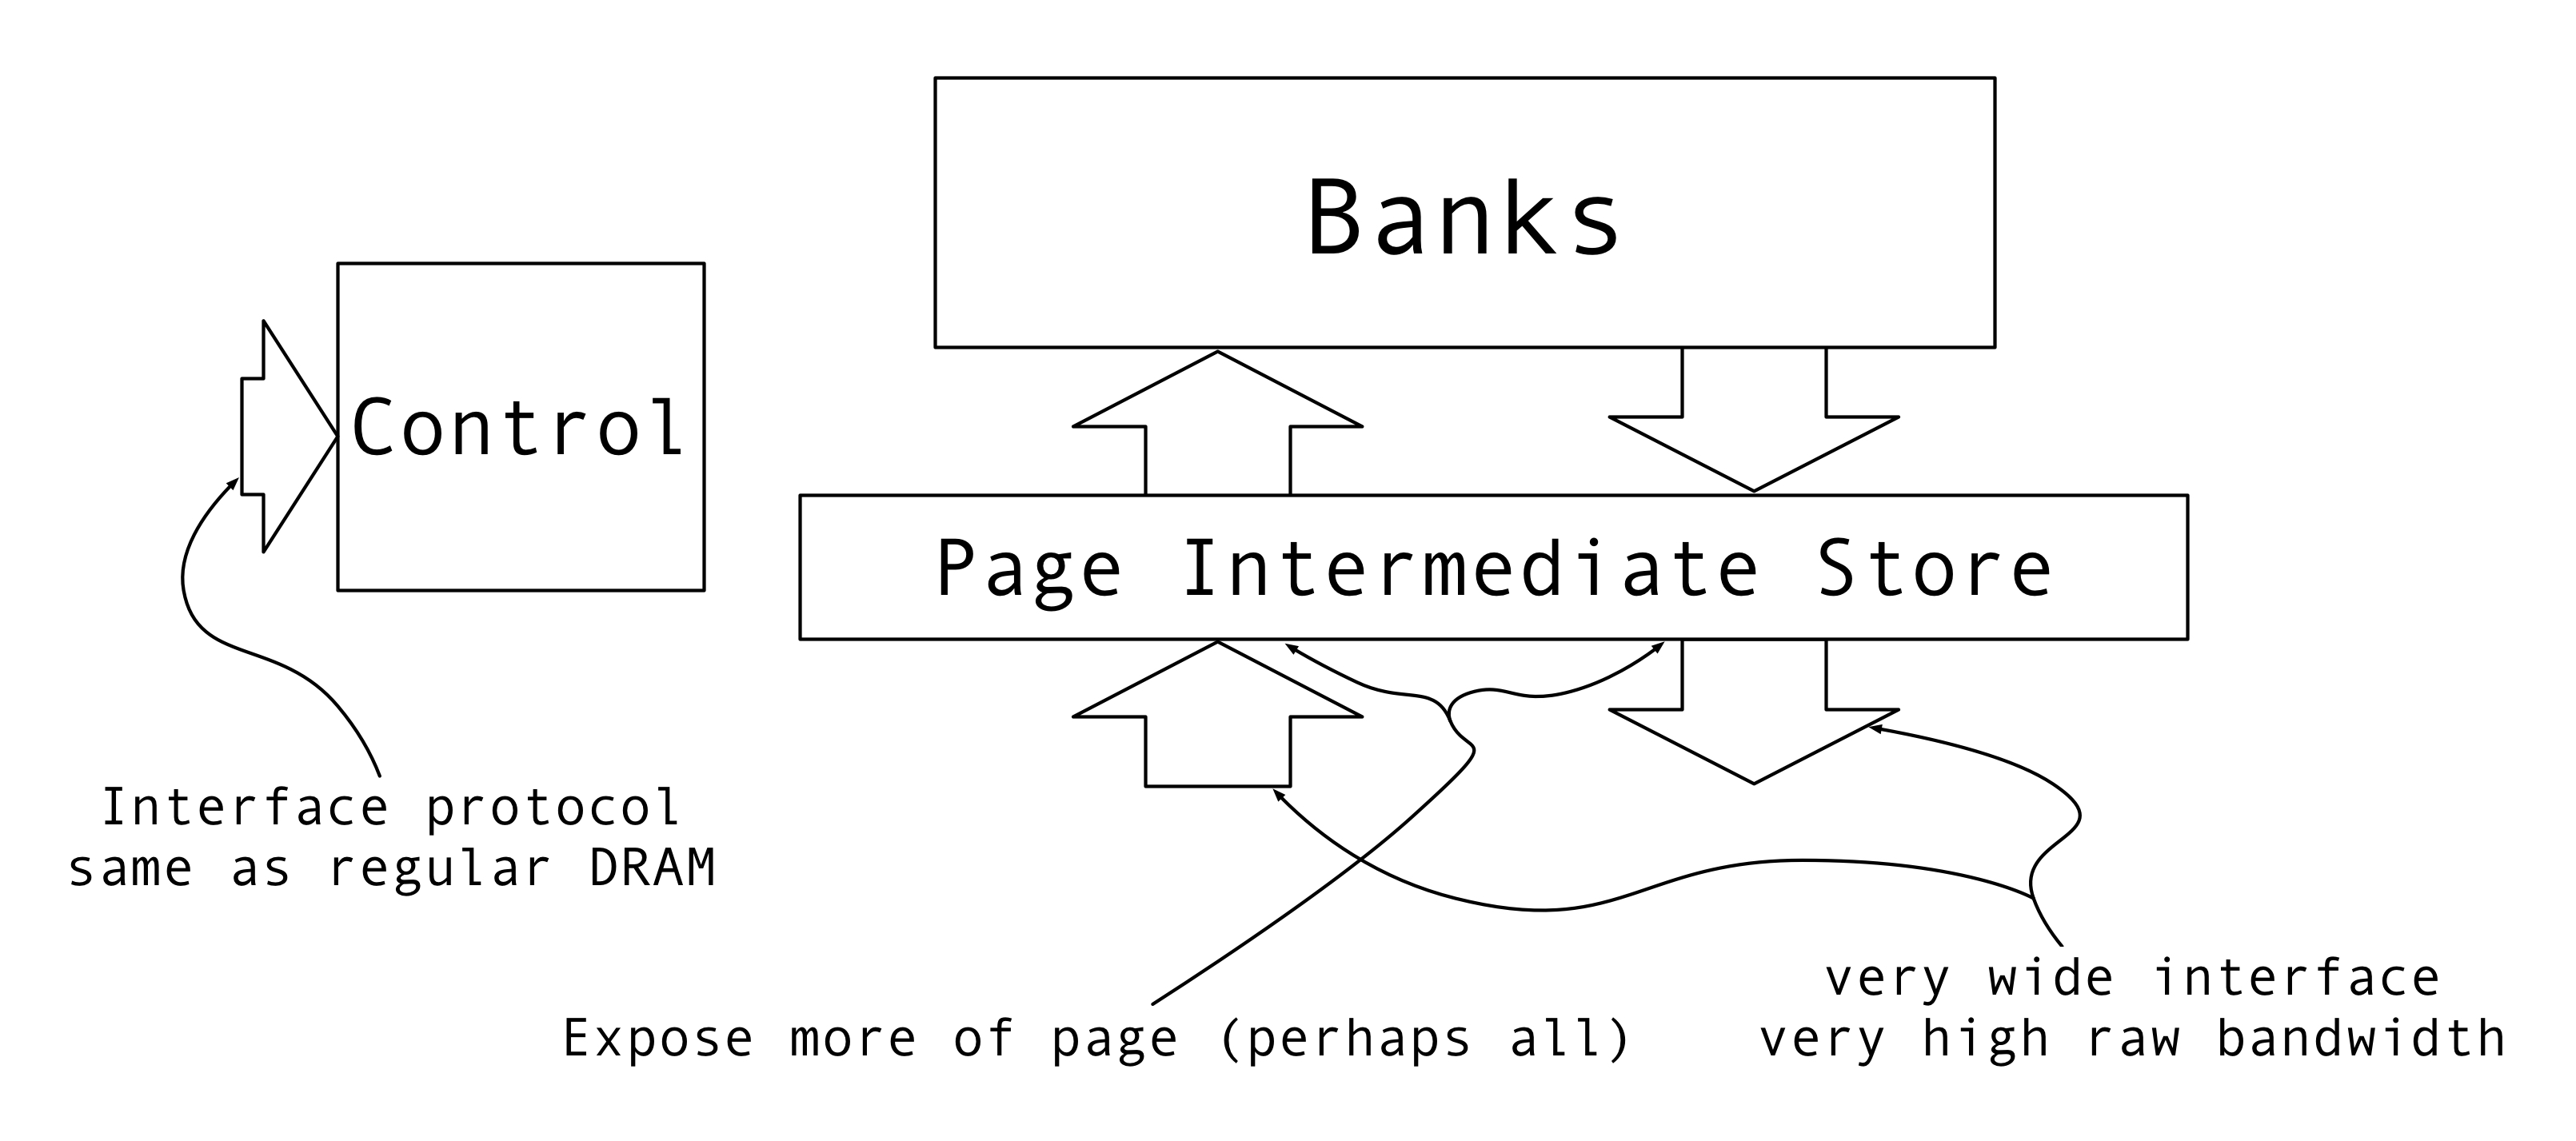
\includegraphics[width=.9\linewidth]{DRAMBusChange.jpg}}
}
\caption{Exposing more of the DRAM page}
\label{fig:dramBusChange}
\end{figure}

\section{Write Mask}
\label{sec:Write Mask}
When processing an ANN, to compute the activation of an individual AN involves reading the pre-synaptic AN activation's and the weights of the connections between the pre-synaptic ANs and the AN being processed. The activation of the processed AN is written back to memory. The ratio of reads to writes is high, 100's or 1000's to one. Therefore, the system often needs to write a portion of the page back to memory. To avoid a read/modify/write, a customization to the DRAM is the addition of a write data mask to the DRAM write path.

